\chapter{Notas de microanálise (MA)} %Anexo F (lista as notas MA e seus respectivos conteúdos)
\label{apendice:f_notas_ma}
\section{Notas de microanálise do Grupo 1 (sem PDTI)}
As páginas a seguir contém as 6 notas do tipo MA criadas durante o desenvolvimento da pesquisa sobre o grupo 1.

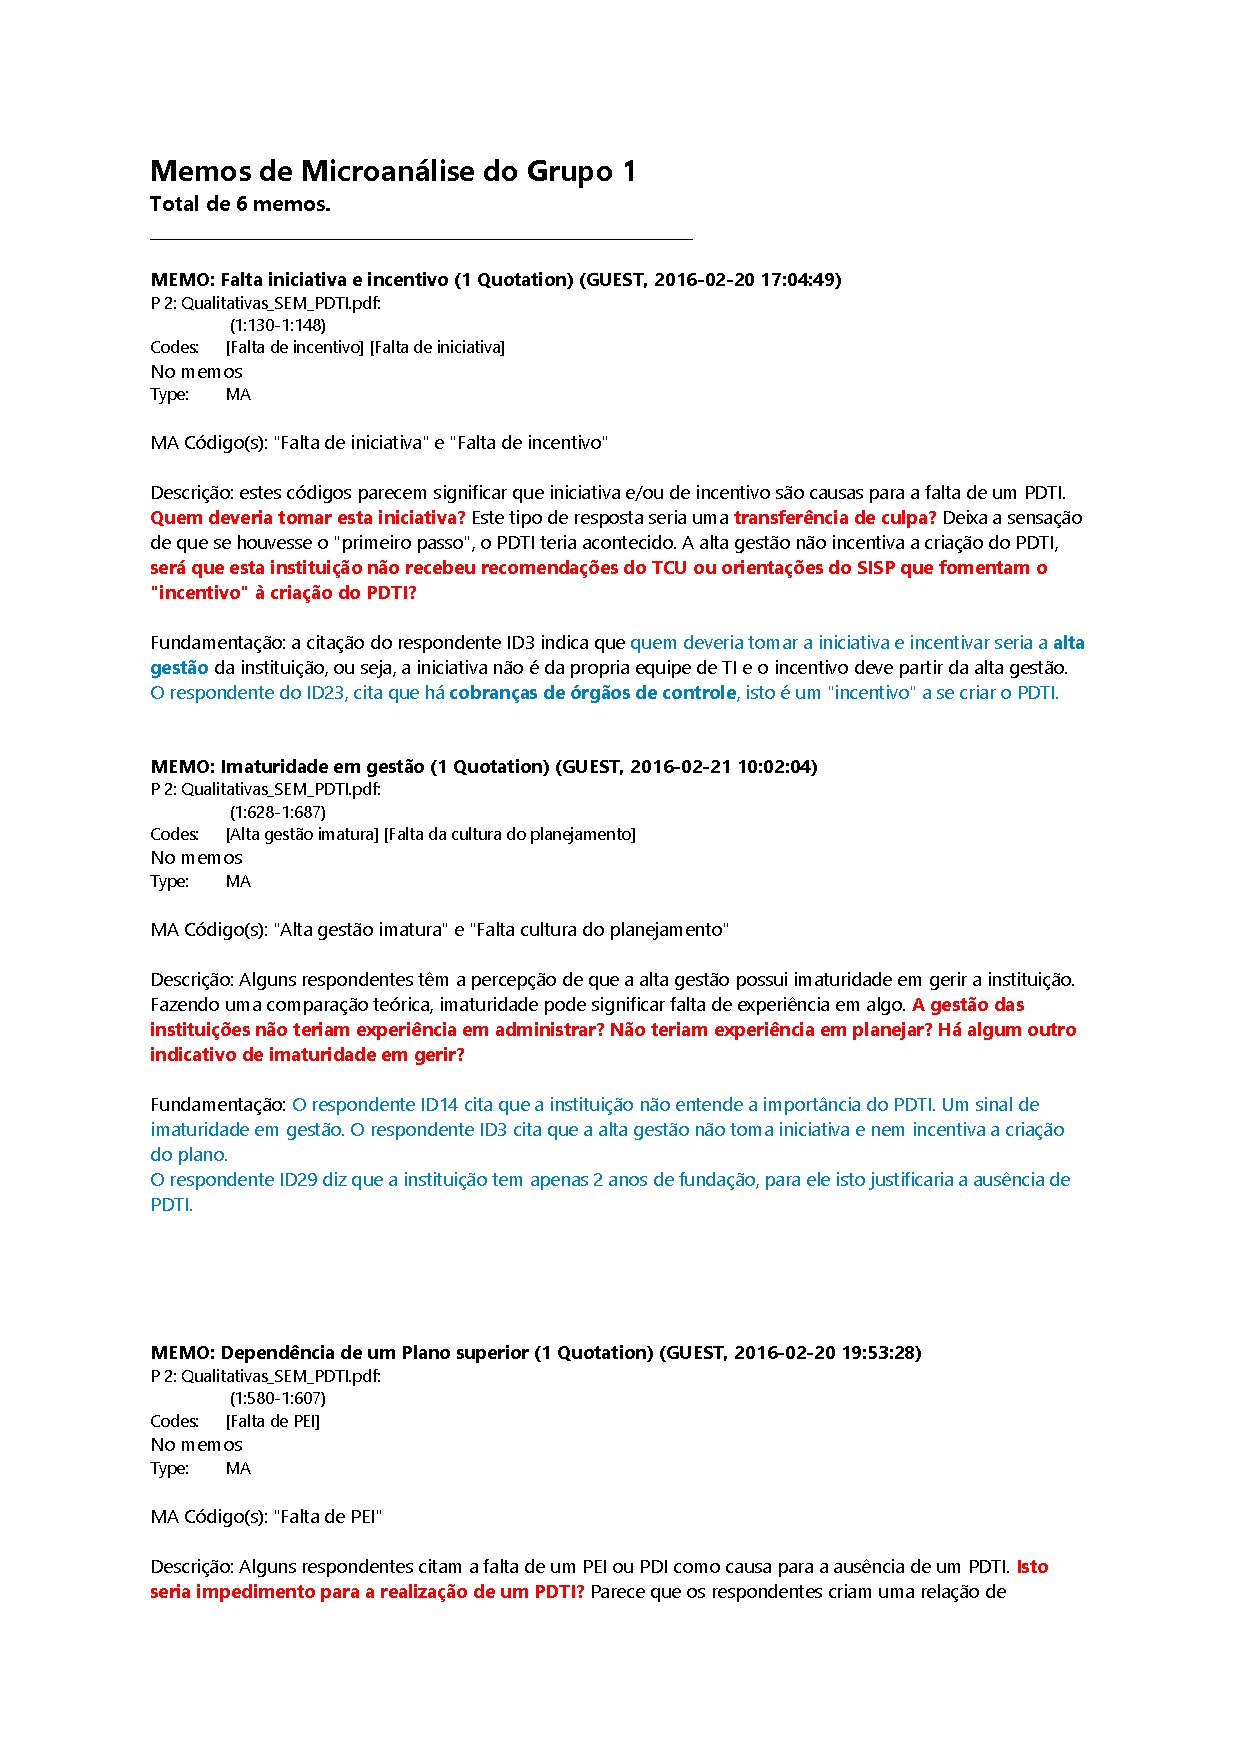
\includepdf[pages=-]{includes/apendiceF_MA_g1.pdf}

\section{Notas de microanálise do Grupo 2 (com PDTI)}
As páginas a seguir contém as 14 notas do tipo MA criadas durante o desenvolvimento da pesquisa sobre o grupo 2.

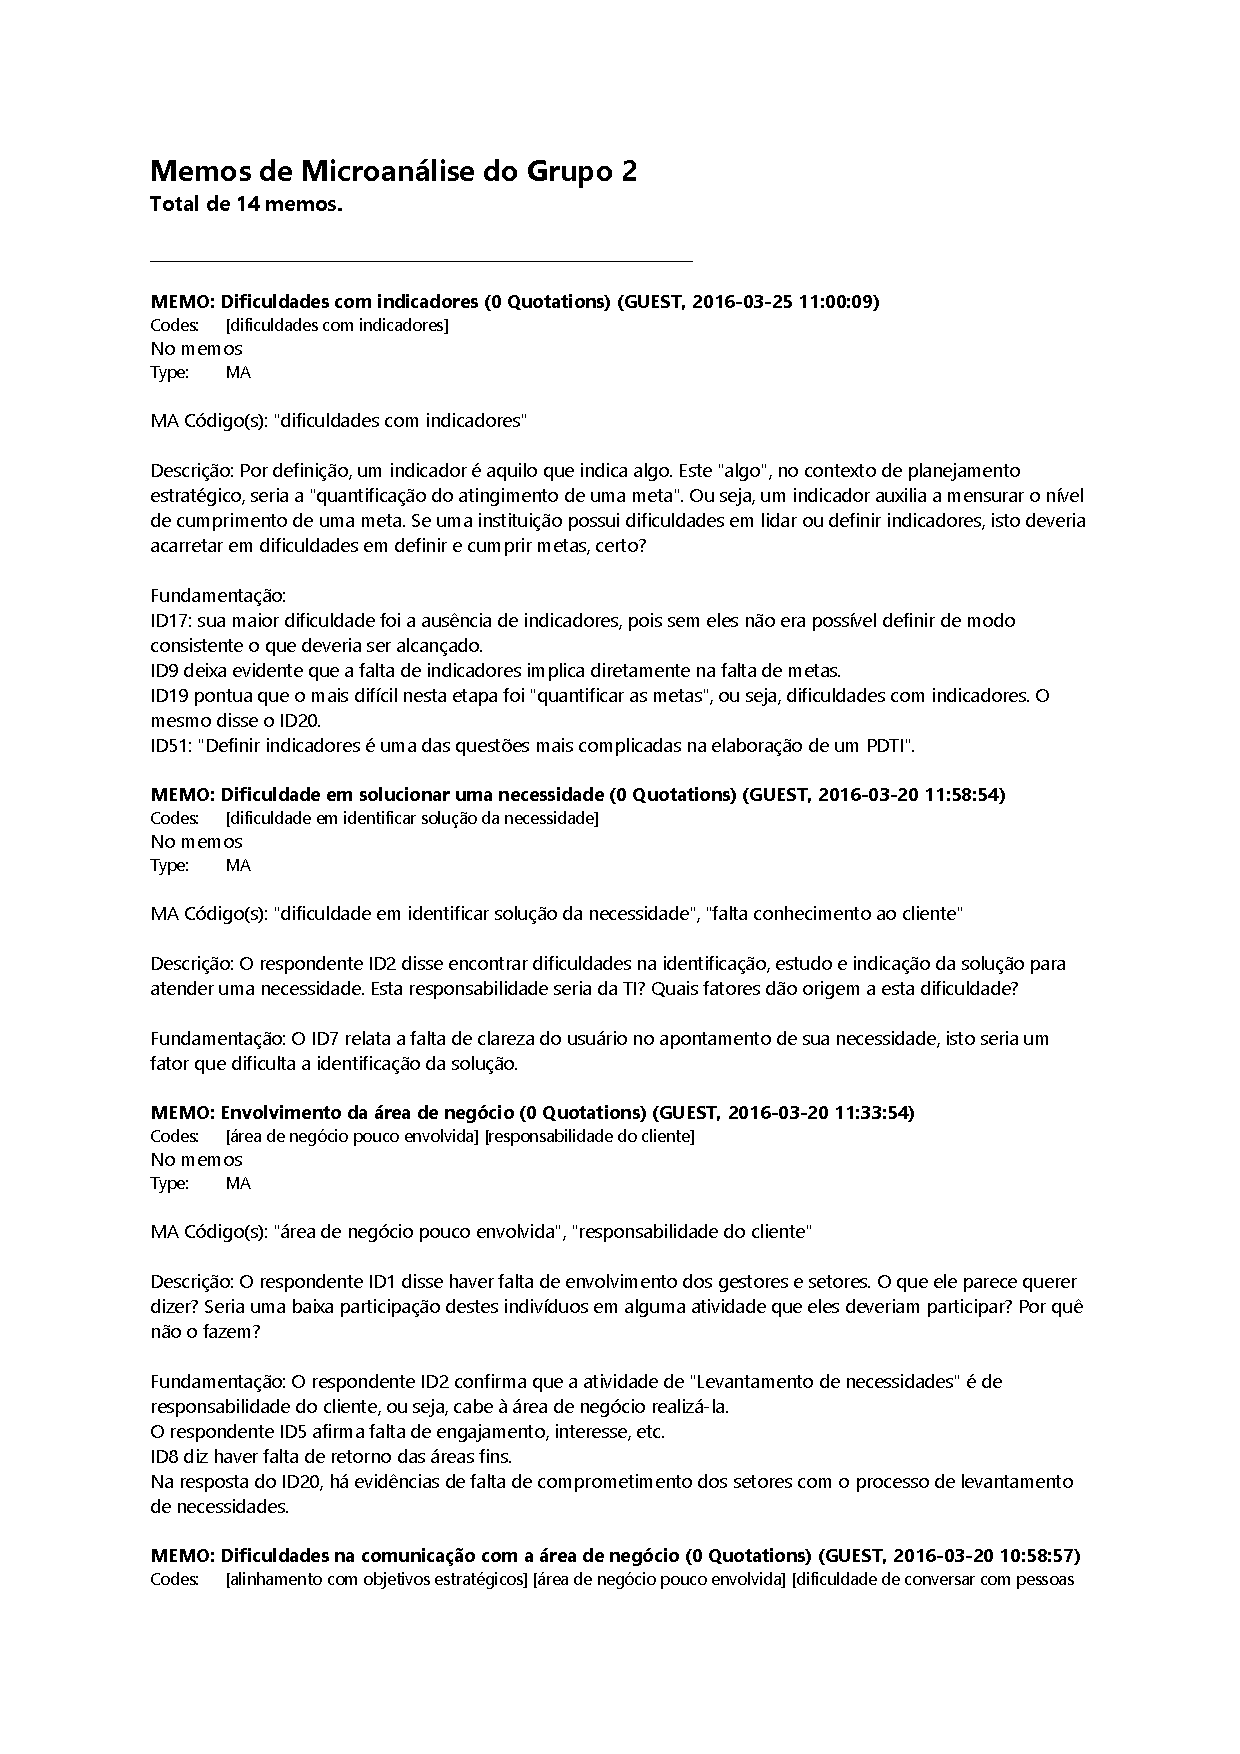
\includepdf[pages=-]{includes/apendiceF_MA_g2.pdf}